\section{Threshold and bootstrap robustness of the K$_3$C$_{60}$ EDT window}

Figure~\ref{fig:s5_threshold_bootstrap} collects the analysis variations used to test the stability of the K$_3$C$_{60}$ curvature-defined EDT window. The nominal configuration is the one used in the main-text K$_3$C$_{60}$ figure: Bands 208 and 209 of mode \texttt{m120}, analysis indices 150--281, local quadratic fit half-window of 18 points, and residual threshold $R_{\rm th}=0.08$. The resulting nominal width is $\Delta k_{\rm EDT}=0.154$.

The first three robustness axes are direct analysis choices. A residual-threshold sweep over $R_{\rm th}\in[0.04,0.18]$ yields widths between 0.137 and 0.178. A fit-window sweep over half-windows from 10 to 28 points yields widths between 0.127 and 0.199. A local-fit bootstrap around the nominal paired branches gives a 95\% confidence interval of $[0.147,\,0.158]$ for the extracted width. These three checks show that the finite window is not created by a single threshold choice or a single local-fit stencil.

The remaining checks probe data-selection sensitivity. Neighboring band-pair choices in the same exported trace produce different finite widths, which is why pair selection is reported explicitly as a robustness axis instead of being hidden inside the nominal workflow. Subsampling the $k$ grid from 131 points to 66, 44, and 33 points changes the width only modestly, to 0.150, 0.144, and 0.164, respectively. The one robustness axis we cannot reproduce from the bundled archive is a displacement-amplitude sweep, because the archive contains one exported curvature dataset rather than a matched family of displaced calculations at several amplitudes. We therefore state this limitation explicitly instead of inferring an unverified amplitude robustness claim.

\begin{figure*}[t]
\centering
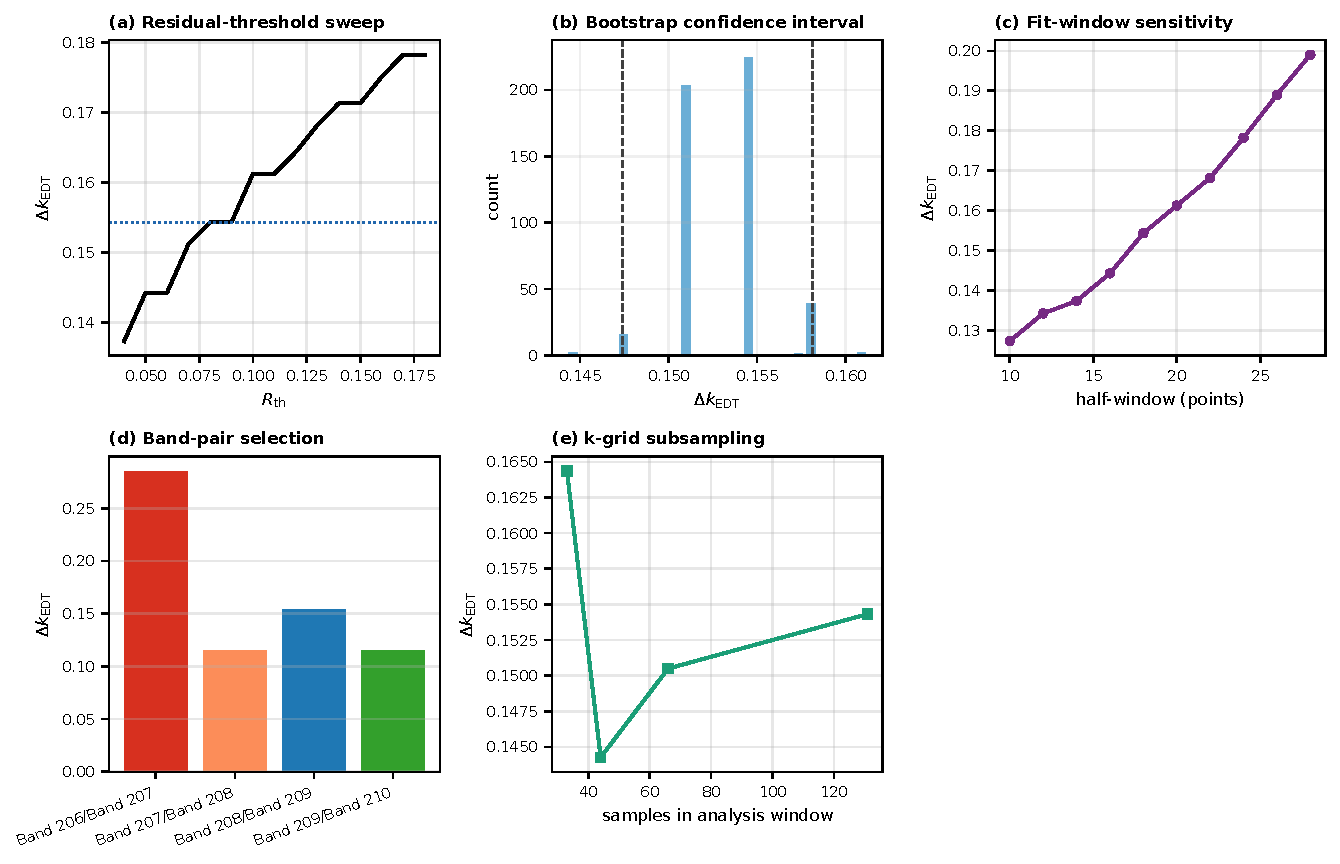
\includegraphics[width=0.94\linewidth]{S5_threshold_bootstrap.pdf}
\caption{\textbf{Robustness checks for the K$_3$C$_{60}$ curvature-defined EDT window.}
(a) Extracted $\Delta k_{\rm EDT}$ as the residual threshold is varied. (b) Bootstrap distribution and confidence interval for the nominal width. (c) Sensitivity to the local quadratic fit half-window. (d) Sensitivity to neighboring band-pair selections in the archived curvature trace. (e) Sensitivity to $k$-grid decimation. (f) Explicit statement of the missing displacement-amplitude sweep in the bundled reproducibility archive.}
\label{fig:s5_threshold_bootstrap}
\end{figure*}
